\begin{align*}
  &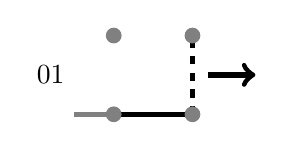
\begin{tikzpicture}[baseline=2.5ex]
    \draw[line width=2, line cap=round, white]
     (-1,0)--(0,0)
     (-1,1)--(0,1)
    ;
    \node at (-0.8,0.5) {$\indxxx 01$};
    \draw[line width=2, gray!100] (-0.5,0)--(0,0);
%
    \draw[line width=2] (0,0)--(1,0);
    \draw[line width=2, dashed] (1,0)--(1,1);
    \fill[gray] (0,0) circle (0.1) (1,0) circle (0.1) (0,1) circle (0.1) (1,1) circle (0.1);
%
    \draw[line width=2, ->] (1.2,0.5)--(1.8,0.5);
  \end{tikzpicture} \set{
  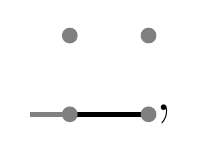
\begin{tikzpicture}[baseline=2.5ex]
    \draw[line width=2, gray!100] (-0.5,0)--(0,0);
    \draw[line width=2] (0,0)--(1,0);
%
    \fill[gray] (0,0) circle (0.1) (1,0) circle (0.1) (0,1) circle (0.1) (1,1) circle (0.1);
    \node at (1.2,0) {\Huge ,};
  \end{tikzpicture}
  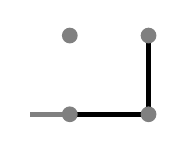
\begin{tikzpicture}[baseline=2.5ex]
    \draw[line width=2, gray!100] (-0.5,0)--(0,0);
%
    \draw[line width=2] (0,0)--(1,0);
    \draw[line width=2] (1,0)--(1,1);
    \fill[gray] (0,0) circle (0.1) (1,0) circle (0.1) (0,1) circle (0.1) (1,1) circle (0.1);
  \end{tikzpicture}
  }
  % = \set{\indxxx 12, \indxxx 01}
% Example 2
  \\
  &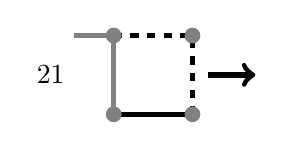
\begin{tikzpicture}[baseline=2.5ex]  % (2, 1) -> (0, 1), (1, 1), (1, 2), (2, 2)
      \draw[line width=2, line cap=round, white]
        (-1,0)--(0,0)
        (-1,1)--(0,1)
      ;
      \node at (-0.8,0.5) {$\indxxx 21$};
      \draw[line width=2, gray!100] (-0.5,1)--(0,1)--(0,0);
%
      \draw[line width=2] (0,0)--(1,0);
      \draw[line width=2, dashed] (0,1)--(1,1)--(1,0);
      \fill[gray] (0,0) circle (0.1) (1,0) circle (0.1) (0,1) circle (0.1) (1,1) circle (0.1);
    \draw[line width=2, ->] (1.2,0.5)--(1.8,0.5);
  \end{tikzpicture} \set{
  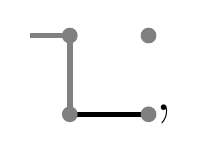
\begin{tikzpicture}[baseline=2.5ex]
    \draw[line width=2, gray!100] (-0.5,1)--(0,1)--(0,0);
    \draw[line width=2] (0,0)--(1,0);
%
    \fill[gray] (0,0) circle (0.1) (1,0) circle (0.1) (0,1) circle (0.1) (1,1) circle (0.1);
    \node at (1.2,0) {\Huge ,};
  \end{tikzpicture}
  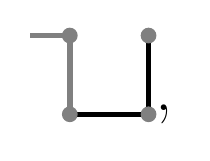
\begin{tikzpicture}[baseline=2.5ex]
    \draw[line width=2, gray!100] (-0.5,1)--(0,1)--(0,0);
    \draw[line width=2] (0,0)--(1,0)--(1,1);
%
    \fill[gray] (0,0) circle (0.1) (1,0) circle (0.1) (0,1) circle (0.1) (1,1) circle (0.1);
    \node at (1.2,0) {\Huge ,};
  \end{tikzpicture}
  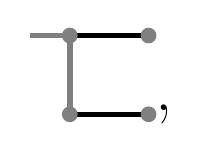
\begin{tikzpicture}[baseline=2.5ex]
    \draw[line width=2, gray!100] (-0.5,1)--(0,1)--(0,0);
    \draw[line width=2] (0,0)--(1,0) (0,1)--(1,1);
%
    \fill[gray] (0,0) circle (0.1) (1,0) circle (0.1) (0,1) circle (0.1) (1,1) circle (0.1);
    \node at (1.2,0) {\Huge ,};
  \end{tikzpicture}
  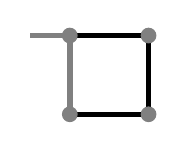
\begin{tikzpicture}[baseline=2.5ex]
    \draw[line width=2, gray!100] (-0.5,1)--(0,1)--(0,0);
    \draw[line width=2] (0,0)--(1,0)--(1,1)--(0,1);
%
    \fill[gray] (0,0) circle (0.1) (1,0) circle (0.1) (0,1) circle (0.1) (1,1) circle (0.1);
  \end{tikzpicture}
  }
\end{align*}